%\documentclass[a4paper]{article} 
\documentclass[final]{IEEEtran}

%\usepackage{nips15submit_09, times}
\usepackage[colorlinks]{hyperref}
\usepackage{url}
\hypersetup{urlcolor={blue}}
\usepackage{amsmath}
\usepackage{algorithm}
\usepackage[noend]{algpseudocode}
\usepackage{graphicx}
\usepackage{cleveref}
\usepackage{amssymb}
\usepackage{eqnarray}
\usepackage{subcaption}
%\usepackage{multicol}
\usepackage{booktabs}
%\usepackage{float}
%\setlength\columnsep{10pt}
\usepackage[margin={.75in,.75in}]{geometry}
\makeatletter
%\usepackage{blindtext} % for dummy text
%\setlength\@fptop{0\p@}
%\makeatother
%\raggedcolumns
\usepackage{etoolbox}
\makeatletter

% \title{Understanding Metropolitan Area Vehicle Movements with Fast, Large-Scale Microsimulation on the GPU\\ or: Metropolitan-Scale Traffic Microsimulation for Agile Planning}

\title{Microsimulation Analysis for Network Traffic Assignment (MANTA) at Metropolitan-Scale for Agile Transportation Planning}

\author{
\large{Pavan Yedavalli}\\
\texttt{University of California, Berkeley}\\
\texttt{\textcolor{black}{pavyedav@berkeley.edu}}\\
\large{Krishna Kumar} \\
\texttt{University of Texas at Austin}\\
\texttt{\textcolor{black}{krishnak@utexas.edu}}\\
\large{Paul Waddell} \\
\texttt{University of California, Berkeley}\\
\texttt{\textcolor{black}{waddell@berkeley.edu}}\\
}

% The \author macro works with any number of authors. There are two commands
% used to separate the names and addresses of multiple authors: \And and \AND.
%
% Using \And between authors leaves it to \LaTeX{} to determine where to break
% the lines. Using \AND forces a linebreak at that point. So, if \LaTeX{}
% puts 3 of 4 authors names on the first line, and the last on the second
% line, try using \AND instead of \And before the third author name.

\begin{document}

\maketitle 

\begin{abstract}
Abrupt changes in the environment, such as increasingly frequent and intense weather events due to climate change or the extreme disruption caused by the coronavirus pandemic, have triggered massive and precipitous changes in human mobility. The ability to quickly predict traffic patterns in different scenarios has become more urgent to support short-term operations and long-term transportation planning, emergency management, and resource allocation. Urban traffic exhibits a high spatial correlation in which links adjacent to a congested link are likely to become congested due to spillback effects. The spillback behavior requires modeling the entire metropolitan area to recognize all of the upstream and downstream effects from intentional or unintentional perturbations to the network. However, there is a well-known trade-off between increasing the level of detail of a model and decreasing computational performance. To achieve traffic microsimulation levels of detail, current implementations often compromise by simulating small spatial scales, such as intersections or corridors that ignore larger network dependencies. These simulators also either require access to expensive high performance computing systems or have computation times on the order of days or weeks that discourage productive research and real-time planning. This paper addresses these performance shortcomings by introducing a new platform, MANTA (Microsimulation Analysis for Network Traffic Assignment), for traffic microsimulation at the metropolitan-scale. MANTA employs a highly parallelized GPU implementation that is fast enough to run simulations on large-scale demand and networks within a few minutes. We test our platform to simulate the entire Bay Area metropolitan region over the course of the morning using half-second time steps. The runtime for the nine-county Bay Area simulation is just over four minutes, not including routing and initialization. This computational performance significantly improves the state of the art in large-scale traffic microsimulation, and offers new capacity for analyzing the detailed travel patterns and travel choices of individuals for infrastructure planning and emergency management.
\end{abstract}
%\begin{multicols}{2}

\section{Introduction}
Rapid global urbanization and an increase in the frequency of extreme events, such as climate change-induced disruptive weather occurrences and global pandemics like COVID-19, are forcing us to re-examine the way we design and improve the resilience of cities, including their transportation infrastructure. Transportation simulation models offer the ability to perform sensitivity analyses and ex-ante evaluation of the impact of potential infrastructure investments~\cite{kokkinogenisNextgenerationTrafficSimulation2011, garcia-doradoDesigningLargescaleInteractive2014, waddellUrbanSimModelingUrban2002}. These simulations explore human mobility patterns, which are motivated by the need to engage in mandatory and discretionary activities. They are carried out on various modes, including walking, biking, driving, or TNC services. The dynamics of traffic flow are affected by factors such as frequency of trips, vehicle occupancy, length of the journeys, route choices, and driving speeds, producing congestion, traffic emissions, and an increase in traffic accidents~\cite{zhaoAgentBasedModelABM}. In addition, certain transportation simulation, such as emergency evacuation planning of a city in an extreme weather event, requires near real-time transportation planning. Hence, to address the need for regional-scale emergency scenarios and broader infrastructure planning by policymakers and urban planners, we develop a fast metropolitan-scale traffic simulation engine capable of characterizing individual behaviors.

Traffic modelers use three alternative types of traffic assignment models to predict the impact of travel demand on the network: (1) macroscopic, (2) mesoscopic, and (3) microscopic, in decreasing order of traveler aggregation and increasing order of granularity~\cite{milamClosingInducedVehicle2017, waraichPerformanceImprovementsLargeScale2015}. Macroscopic models are based on the continuum assumption in classical fluid mechanics. The traffic flow is treated as continuous, similar to a flow of a liquid in a pipe, rather than that comprising of discrete vehicles~\cite{maerivoetTransportationPlanningTraffic2005a}.  These macroscopic models are useful in analyzing traffic systems covering a wide area, often across regions, and on highways where the overall speed dictates the macroscopic changes~\cite{kokkinogenisNextgenerationTrafficSimulation2011}. Unlike macroscopic models that assume a continuous vehicular flow on the road link (edge), mesoscopic models employ aggregated volume delay functions, by clustering a set of vehicles into packets and evaluating the movement of these clusters~\cite{kokkinogenisNextgenerationTrafficSimulation2011}. In contrast to these models, microscopic traffic simulation models provide even greater granularity, giving explicit consideration to the interactions between individual vehicles within a traffic stream and employing characteristics such as vehicle lengths, speeds, accelerations, time, and space headways~\cite{toledoMicroscopicTrafficSimulation2005}. 

Regional-scale transportation modeling has been dominated by the macroscopic and mesoscopic models, due to their relative computational efficiency and familiarity~\cite{kotusevskiReviewTrafficSimulation2009}. However, one of the significant drawbacks of these simulators is their lack of granularity. They are limited by the accuracy of representing real-world vehicle dynamics, especially in congested regimes and for emergency scenarios~\cite{toledoMicroscopicTrafficSimulation2005, axhausenActivityBasedApproaches1992}. Traffic flow dynamics are naturally an outcome of the interaction of a many-particle system, where each particle exhibits different characteristics~\cite{yangMicroscopicTrafficSimulator1996}. Only a microsimulation model can capture these intricacies of individual components and complex interactions with reasonable accuracy~\cite{loderUnderstandingTrafficCapacity2019, yangMicroscopicTrafficSimulator1996, toledoMicroscopicTrafficSimulation2005, geroliminisIdentificationAnalysisQueue2011}. However, microsimulation has a high computational cost due to the granularity required in simulating of vehicle movements. Hence, regional-scale microsimulation has generally been impractical~\cite{saidallahComparativeStudyUrban2016, kokkinogenisNextgenerationTrafficSimulation2011}. Although many traffic simulators exist, such as MATSim, SUMO, AIMSUN, Polaris, TRANSSIM, VISSIM, and DynaMIT, among others, these simulators are not designed to tackle large-scale traffic microsimulation efficiently~\cite{Horni2016, dlr46740, barceloDynamicNetworkSimulation2005, auldPOLARISAgentbasedModeling2016, saxenaProblemSolvingUncertainty2016, parkMicroscopicSimulationModel2003, ben-akivaDynaMITSimulationbasedSystem1998}. As a result, techniques such as sampling a small fraction of the transportation demand are currently employed to achieve regional-scale traffic models in a reasonable amount of time and computational cost.

This paper introduces a massively parallelized GPU implementation of a metropolitan-scale microsimulation engine - MANTA. MANTA is an agile regional-scale microsimulator capable of efficiently simulating over 7 million agents at a spatial scale as large as the San Francisco Bay Area, in under 10 minutes. First, we present the components of the simulation, then the mathematical theory and implementation of the simulator, followed by the results of a case study in the Bay Area. We then present the calibration and validation of the simulator, performance benchmarks, limitations and future work, and finally the conclusions.

\section{Components}
The objective of this study is to perform a regional-scale microsimulation of vehicular traffic of the Bay Area, incorporating individual trips on a typical workday morning. The microsimulator builds on the initial implementation by~\cite{garcia-doradoDesigningLargescaleInteractive2014, waddellIntegratedPipelineArchitecture2018}. In this section, the network generation, demand creation, routing, and simulation architectures are described in detail. 

%Specifically, the method to generate the street network are determined and generated. Real-world travel demand is then retrieved in a given time slice from the local metropolitan transit organization, Bay Area MTC. From this demand, the origin and destination nodes of each trip are parsed, allowing for calculating the shortest-path for the individual to traverse the network from origin to destination. After computing the shortest-path, the microsimulation randomly generates the timing of trips across a specific range of time and models the precise vehicle behavior on each edge as all individuals traverse the network, reflecting real-world dynamics at a high level of detail.

\subsection{Street Network}

For the case study, we use the San Francisco Bay Area, which includes nine counties. The street network is constructed from the OpenStreetMap (OSM) network within the polygonal hull of the counties in the metropolitan area using the OSMnx library~\cite{boeingOSMnxNewMethods2017a}. The network contains all roads in the Bay Area, from large primary roads to tertiary streets. The OSM network currently considers points representing curves or bends in edges to be nodes, which is not topologically accurate for network analysis~\cite{waddellIntegratedPipelineArchitecture2018, boeingOSMnxNewMethods2017a}. Hence, the network topology is simplified by retaining only those nodes at intersections and dead-ends. The simplified network topology results in a fully-connected network, in which all nodes in the network are connected to at least one other node in the network. There are no hanging nodes without a path.~\Cref{fig:bay_area_edges} shows the full network with 224,223 nodes and 549,008 edges. The number of lanes, length, and free-flow speeds for each edge are then extracted from OSM data or imputed. The speed limit of each edge is taken from OSM if available; if not, a free-flow speed based on the edge's number of lanes, and the type of road is derived and then used as the edge's speed limit. If the number of lanes is not available, then a recommended default value from OSM is used depending on the type of road. For instance, a tertiary road without a specified number of lanes is given a default speed limit of 20 mph, and a motorway without a specified number of lanes is given a default speed limit of 57.5 mph.


% \begin{figure}[H] 
% 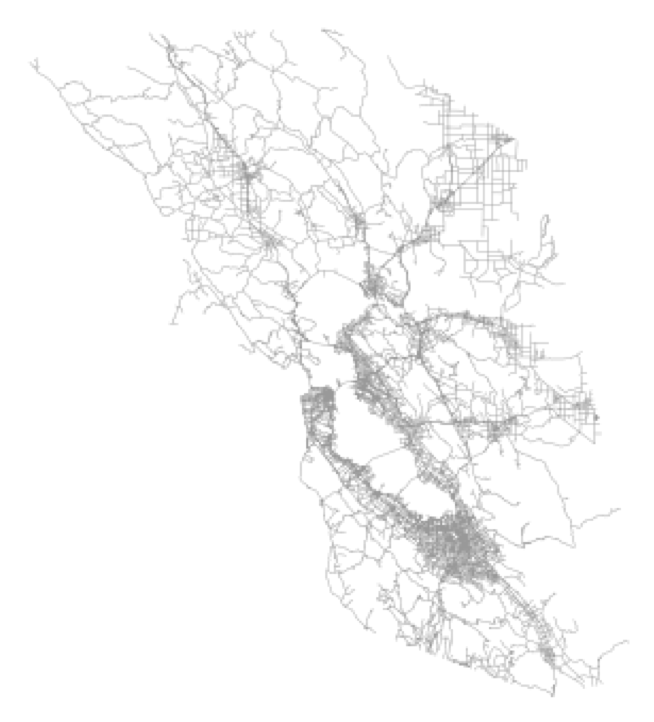
\includegraphics[width=.45\textwidth]{figs/edges.png}
% \caption{The Bay Area edges}
% \label{fig:bay_area}
% \end{figure}

\begin{figure}
    \centering
    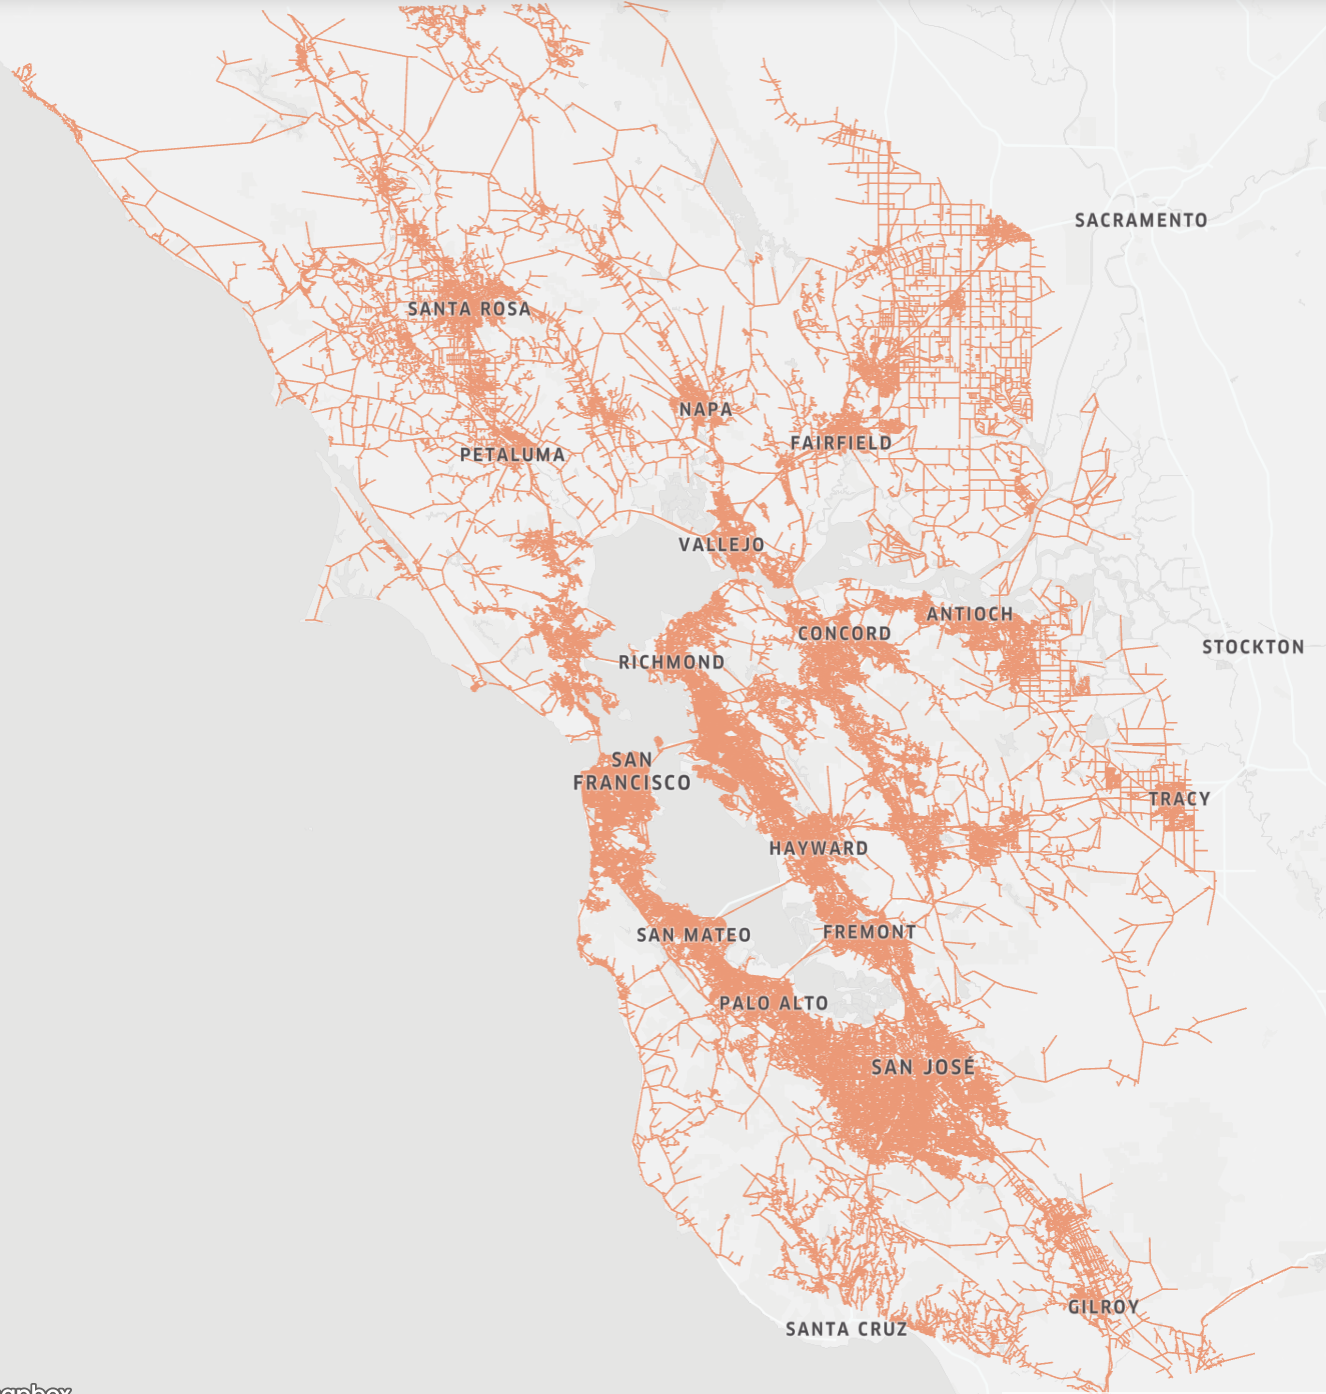
\includegraphics[width=.45\textwidth]{figs/bay_area_edges_kepler.png}
    \caption{The Bay Area Network with 224,223 nodes and 549,008 edges}
    \label{fig:bay_area_edges}
\end{figure}

\subsection{Demand}

The origin-destination (OD) demand is derived from data generated by the Bay Area Metropolitan Transportation Commission (MTC) travel model. The trips are narrowed to morning trips between 5 AM and 12 PM and further restricted to automobile trips, which consist of both driving and TNC trips.

The OD pairs are available at the granularity of traffic analysis zones (TAZ). Thus, individual trips must be mapped to specific network nodes within the TAZ polygon. First, all the nodes of the street network are assigned to their respective TAZ polygon. After mapping nodes to their TAZs, each origin and destination is randomly assigned to one of the TAZ nodes. This process differs from \cite{waddellIntegratedPipelineArchitecture2018}, where each origin or destination is assigned to the centroid of the respective TAZ. Given that microsimulation models individual vehicle behavior, adding diversity of nodes to the simulation, rather than using the same node for every trip that contains the same origin or destination TAZ, is expected to mimic travel patterns more realistically. The final OD demand has 3,269,864 travelers.

%From this, there exist 91 TAZs, out of a total of 1454, in the Bay Area that did not have any nodes, due to geography or long edges. 

\subsection{Routing}
After generating the network and the corresponding OD demand, the next step of the simulation is to compute the shortest-path between each origin and destination. Shortest-path algorithms have been bottlenecks in many traffic models, requiring either significant pre-processing time or great computational cost~\cite{dellingEngineeringRoutePlanning2009a}. The initial implementation of the microsimulator used Johnson's shortest-path algorithm, an all-pairs shortest-path (APSP) technique. APSP involves computing the shortest-path using Dijkstra's algorithm for all possible pairs of node connections in a network. This produces a $N \times N$ matrix that must be stored in memory (RAM), where $N$ is the total number of nodes in the network~\cite{garcia-doradoDesigningLargescaleInteractive2014}. However, the memory requirement grows significantly as $N^2$. For the Bay Area network with 224,223 nodes, the memory required to compute APSP is 402 GB, making it extremely memory intensive for accessible computing hardware. However, Johnson's algorithm remains valuable after this initial overhead of calculating the all-pairs shortest-path, as future queries of the shortest-path would be a lookup with constant time, $O(1)$. 

%However, this would also remain an issue in dynamic routing. As traffic traverses the network, the shortest-path has to be computed at the end of each time step, which undermines the usefulness of the constant lookup ability of Johnson's algorithm. Besides, the memory requirement makes Johnson's algorithm unusable on a standard CPU.
As a result, one of the significant contributions of this paper is the integration of a parallelized Dijkstra's priority queue single-source shortest-path (SSSP) algorithm, described in \cite{zhaoAgentBasedModelABM}, in which only the OD pairs required in the simulation are computed. Typically, the number of agents $n$ and their paths are significantly smaller than the APSP $O(N^2)$. The priority-queue algorithm is parallelized with a hybrid MPI/OpenMP scheme, which allows for linear scaling with millions of agents. An open addressing scheme-based hashmap is used to store key-value pairs of edge weights, hence updating the edge weights during the simulation and computing the shortest-path becomes more efficient. This open addressing scheme improves the performance of hashmaps by 20\%, providing quicker access to edges and connectivity. A simulation with 3.2 million OD pairs routes on the large Bay Area network is calculated within 62 minutes on an Intel I9 processor with 2 threads per core and 14 cores per socket. This is a significant improvement from the prior APSP implementation, which could not be run due to its massive memory requirements.


\subsection{Microsimulation}

The microsimulation framework we adopt is an enhanced and extended version of the architecture developed by~\cite{garcia-doradoDesigningLargescaleInteractive2014}. The vehicles move in discrete timesteps of $\delta t = .5$ seconds, following the state of the art microsimulators today~\cite{dowlingTrafficAnalysisToolbox2004}. The simulation described in this paper is carried out from 5 AM to 12 PM to model a typical morning workday. Each traveler in the OD demand is randomly assigned a departure time within this specified range by sampling from a normal distribution that roughly mimics the morning peak-hour behavior, with a peak around 7:30 AM and a standard deviation of 45 minutes. The departure time specified for individual vehicles in the simulation is presented in~\Cref{fig:dep_times}.

\begin{figure}
    \centering
    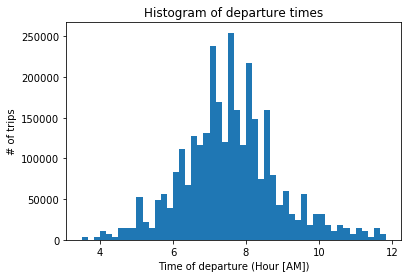
\includegraphics[width=.45\textwidth]{figs/departure_times.png}
    \caption{Departure times are chosen between 5 AM to 12 PM to model the morning hours. It follows a Gaussian distribution in which the bulk of the trips begin between 6:30 AM and 8:30 AM.}
    \label{fig:dep_times}
\end{figure}

At each timestep, the vehicle's travel time, position, and velocity are updated. MANTA employs a unique traffic atlas concept, akin to a texture atlas in the computer graphics community or a discretization step in signal processing. Each road segment is assigned a contiguous set of bytes in memory, where each byte represents $t_m$ meters of a lane and can be occupied by at most one vehicle~\cite{garcia-doradoDesigningLargescaleInteractive2014}. This byte of data stores the car's speed~\cite{garcia-doradoDesigningLargescaleInteractive2014}. Hence, cars on the same edge are located on adjacent bytes of memory. The traffic atlas significantly reduces the computational cost of finding neighboring vehicles, as it involves only looking up the status of neighboring cells in memory, instead of a complex spatial distance query, thus enabling GPU parallel computation.~\cite{garcia-doradoDesigningLargescaleInteractive2014}. 

In MANTA, the vehicular movement on an edge is dictated by conventional car following, lane changing, and gap acceptance algorithms \cite{toledoMicroscopicTrafficSimulation2005}. The well-known Intelligent Driver Model (IDM), as shown in~\Cref{eq:idm}, is used to control the vehicle dynamics through the network \cite{treiberTrafficFlowDynamics2013}.
\begin{equation} 
    \dot{v} = a (1 - (\frac{v}{v_o})^\delta - (\frac{s_o + Tv + \frac{v\Delta v}{2\sqrt{ab}}}{s})^2)
    \label{eq:idm}
\end{equation}
where $\dot{v}$ is the current acceleration of the vehicle, $a$ is the maximum possible acceleration of the vehicle, $v$ is the current speed of the vehicle, $v_o$ is the speed limit of the edge, $\delta$ is the acceleration exponent, $s$ is the gap between the vehicle and the leading vehicle, $s_0$ is the minimum spacing allowed between vehicles when they are at a standstill, $T$ is the desired time headway, and $b$ is the braking deceleration of the vehicle \cite{garcia-doradoDesigningLargescaleInteractive2014, waddellIntegratedPipelineArchitecture2018}. The exact position of each vehicle at the current timestep is computed using this calculated acceleration value $\dot{v}$.

The IDM contains several parameters that are calibrated for the current case study using observed data. Simulations from~\cite{treiberTrafficFlowDynamics2013} were used to determine the ranges used in calibration for $a$, $b$, $T$, and $s_0$, shown in~\Cref{tab:idm_params}.
\begin{table}   
    \centering
    \begin{tabular}{ l  c  c }
        \toprule
         Parameter & Value & Units \\
         \midrule
         $a$ & $\mathcal{N}(1,10)$ & $\frac{m}{s^2}$ \\  
         $b$ & $\mathcal{N}(1,10)$ & $\frac{m}{s^2}$ \\
         $T$ & $\mathcal{N}(.1,2)$ & $s$ \\
         $s_0$ & $\mathcal{N}(1,5)$ & $m$\\
         \bottomrule
    \end{tabular}
    \label{tab:idm_params}
    \caption{IDM parameter ranges, derived from ~\cite{treiberTrafficFlowDynamics2013}}
\end{table}
In addition to car following, vehicles can also change lanes within an edge. There are two types of lane changes: mandatory and discretionary~\cite{garcia-doradoDesigningLargescaleInteractive2014}. Mandatory lane changes occur when the vehicle must take an exit off the road, while discretionary lane changes occur during overtaking or voluntary movements~\cite{garcia-doradoDesigningLargescaleInteractive2014}. The lane changing model gives the vehicle an exponential probability from switching from a discretionary lane change to a mandatory lane change, as shown in~\Cref{eq:lane_changing}.
\begin{equation}
    m_i = 
    \begin{cases} 
        e^{-(x_i - x_0)^2} & x_i \geq x_0 \\
        1 & x_i \leq x_0
        \label{eq:lane_changing}
    \end{cases}
\end{equation}
where $m_i$ is the probability of a mandatory lane change for vehicle $i$, $x_i$ is the distance of vehicle $i$ to an exit or intersection, and $x_0$ is the distance of a critical location to the exit or intersection~\cite{iqbalDevelopmentOriginDestination2014a, yangMicroscopicTrafficSimulator1996}. Intuitively, as the vehicle travels further along in a path, its probability of making a lane change to make a turn or exit increases. Once a vehicle has decided to change lanes, the maneuver is performed if the lead and lag gaps are acceptable. The critical lead or lag gap for a successful lane change are defined as the minimum distance to the following or lagging vehicle at which a lane change can be performed, respectively, as shown in~\Cref{eq:gap}.
\begin{align}
    \label{eq:gap}
    g_{lead} &= \max(g_a, g_a + \alpha_{a1}v_i + \alpha_{a2}(v_i - v_a)) + \epsilon_a  \\ 
    g_{lag} &= \max(g_b, g_b + \alpha_{b1}v_i + \alpha_{b2}(v_i - v_b)) + \epsilon_b
\end{align}

where $g_{lead}$ is the critical lead gap for a lane change, $g_{lag}$ is
the critical lag gap for a lane change, $g_a$ is the desired lead gap for a lane change, $g_b$ is the desired lag gap for a lane change, $\alpha$ is a system parameter (typically [0.05,0.40]) that controls the gap based on speed, $v_i$ is the speed of the vehicle, $v_a$ is the speed of the lead vehicle, $v_b$ is the speed of the lag vehicle, and $\epsilon_a$ and $\epsilon_b$ are the random components~\cite{garcia-doradoDesigningLargescaleInteractive2014}.

The representation and modeling of intersections in this initial application of the traffic simulator is simplistic and not representative of diverse real-world dynamics at intersections. We consider two different types of traffic control. Case 1 traffic control is a flashing red light at each node, where only one vehicle can move into the intersection at a particular time. If the node contains $n$ inbound edges and $m$ outbound edges, the system will create a round-robin of the $nm$ combinations for all cars to pass through the intersection based on their position in their lane queue~\cite{waddellIntegratedPipelineArchitecture2018}. Case 2 traffic control assigns every node as a green light, where all cars pass through with no delay. This is clearly not realistic for most nodes that have stop signs or traffic lights, but is plausible for nodes along highway interchanges. These two different conditions produce surprisingly realistic overall results despite the simplification in the intersection control. The results are discussed later in this paper. Future work includes the ability to infer the correct traffic control at every intersection using deep learning techniques.

%In summary, for each active vehicle, several calculations are performed. The distance to the following vehicle is first calculated. If there is no following vehicle, the distance to the intersection and type of traffic control at the intersection is determined. If it is a red light (case 1), the car will wait its turn relative to the intersection queue of cars to pass through the intersection with its $v = 0$. If it is a green light (case 2), it moves through the intersection with no regard for possible collisions at the intersection. Then, the vehicle's position, acceleration, and velocity are updated based on the previous governing equations. 

\section{Shortest-path results}
Preliminary travel patterns already emerge from the initial shortest-path calculation.~\Cref{fig:volume} displays a log histogram of edge volumes across the network, showing that the bulk of edges have vehicle counts below 1000 and are traversed infrequently. Only a small fraction of the edges account for the majority of the most frequently traversed routes.
\begin{figure} 
    \centering
    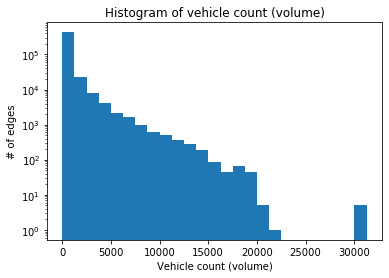
\includegraphics[width=.45\textwidth]{figs/vehicle_counts_on_edges_log_y_axis.png}
    \caption{Histogram (log y-axis) showing the number of edges that see a particular vehicle count across the time range simulated. Most edges see fewer than 100 vehicles in the timeframe}
    \label{fig:volume}
\end{figure}
Routes across the Bay Bridge are shown in~\Cref{fig:transbay}. Unsurprisingly, the Bay Bridge remains a unique outlier, as it produces the maximum volume at 31270 vehicles in the seven-hour duration. From ~\cite{actransitBayBridgeCorridor2010} by AC Transit and ARUP, 41727 trips out of a total of approximately 4M trips traverse the Bay Bridge between 5 AM and 12 PM, representing 1\% of all trips. This proportion of Bay Bridge traversals matches the proportion from the microsimulation at roughly 0.98\% (31270 trips out of 3.2M total trips in the Bay Area).

% \begin{figure} 
% 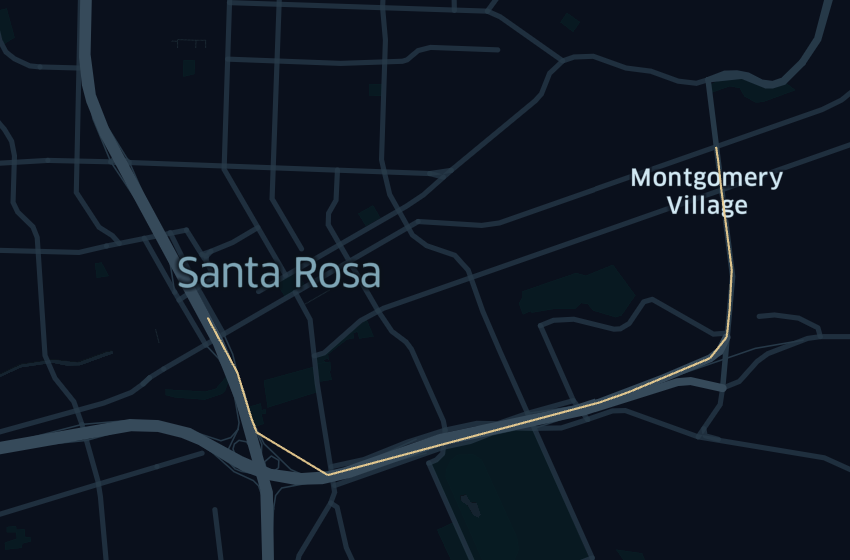
\includegraphics[width=.45\textwidth]{figs/santa_rosa.png}
% \caption{Sample route in Santa Rosa, CA}
% \label{fig:santa_rosa}
% \end{figure}

% \begin{figure}[H] 
% 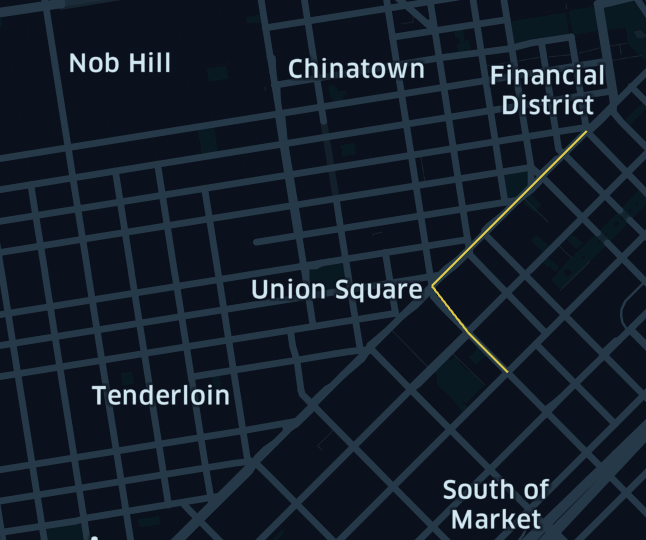
\includegraphics[width=.45\textwidth]{figs/sf_route.png}
% \caption{Sample route in San Francisco, CA}
% \label{fig:sf}
% \end{figure}

\begin{figure} 
    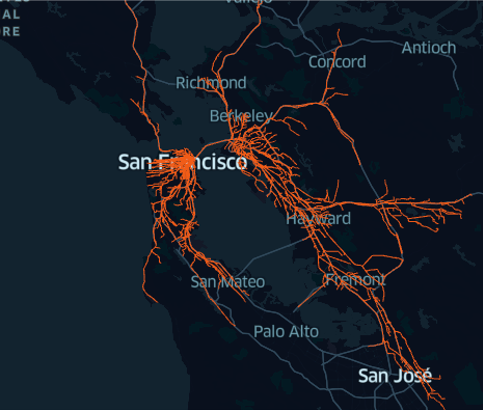
\includegraphics[width=.45\textwidth]{figs/bay_bridge_trips.png}
    \caption{All routes across the Bay Bridge}
    \label{fig:transbay}
\end{figure}

\section{Simulation results}

Infrastructure and scenario planning requires a high degree of accuracy in modeling the vehicle dynamics. This section highlights the calibration and validation techniques along with the microsimulator results. Previous studies have relied on vehicle counts, queue lengths at intersections, and vehicle speeds at loop detectors as ground truth data for calibration and validation \cite{technicalactivitiesdivisionDynamicTrafficAssignment2011}. In this work, we adopt novel approaches of calibration and validation using granular GPS tracking from Uber Movement data, which includes velocities of different edges over time.

\subsection{Calibration}
Traffic microsimulators require calibration to real-world data to adequately represent observed dynamics across a wide range of the network~\cite{barceloDynamicNetworkSimulation2005}. As previously mentioned, in the IDM, parameters $a$, $b$, $T$, and $s_0$ are require calibration. The objective of the calibration process is to minimize the sum of the errors between every edge's speed from MANTA and the Uber data (L1 norm). This optimization problem is specified in~\Cref{eq:calibration}.
\begin{equation}
    \min_{a,b,T,s_0}{\sum_{n=1}^N}{|\frac{\sum_{k=1}^K{\dot{v_k}t}}{K} - \overline{v}{_{uber}}|}
    \label{eq:calibration}
\end{equation}
where $v = \dot{v}t$, $a$ is the acceleration, $b$ is braking, $T$ is time headway, $s_0$ is the linear jam distance, $\delta$ is the exponent of the IDM, $K$ is the number of cars on each edge, $N$ is the number of edges that were successfully matched between Uber's data and MANTA data. Expanding further in~\Cref{eq:calibration_full},
\begin{equation}
    \min_{a,b,T,s_0}{\sum_{n=1}^N}{\frac{\sum_{k=1}^K{\dot{[a(1 - (\frac{v_k}{v_{0,n}})^\delta - (\frac{s_o + Tv + \frac{v\Delta v}{2\sqrt{ab}}}{s})^2]}t}}{K} - \overline{v}{_{uber}}|}
    \label{eq:calibration_full}
\end{equation}
where, as previously specified, $a$ is the acceleration potential, $b$ is the braking potential, $T$ is time headway, and $s_0$ is the linear jam distance.

Given the highly nonlinear nature of the objective function, a numerical method is used. We constrain $a$ and $b$ to $[1,10]$ meters per second squared, $T$ to $[0.1,2]$ seconds, and $s_0$ to $[1.0,5.0]$ meters, and set $\delta$ to 4, the standard exponent of the IDM~\cite{treiberTrafficFlowDynamics2013}. A mini-batch gradient descent is then carried out, with each iteration executing runs for 5 different sets of {$a$, $b$, $T$, and $s_0$}. After simulating every new set, we gathered the sum of every edge's delta in speed between MANTA and Uber, represented by $\frac{\sum_{k=1}^K{\dot{v_k}t}}{K}$. The goal is to find the set {$a$, $b$, $T$, $s_0$} that minimizes this sum of differences. The set that produces the lowest mean difference is chosen as the nominal vector for the next iteration. Each parameter is then perturbed by a value chosen randomly in the range $[-1,1]$. The calibration process converges once the mean difference decreases below a particular threshold. This threshold was chosen to be $.05$ miles per hour due to calibration runtime limitations. As shown in~\Cref{fig:calibration}, the calibration process converged after five iterations.

\begin{figure}
    \centering
    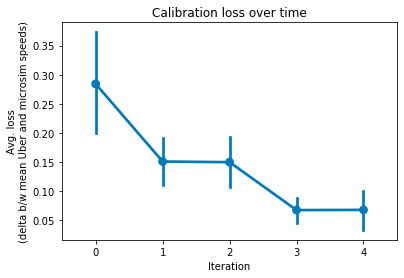
\includegraphics[width=.45\textwidth]{figs/calibration.png}
    \caption{The calibration process: average mean difference between Uber and MANTA speeds over time}
    \label{fig:calibration}
\end{figure}

\subsection{Validation}
% Validating case 2 against Uber Movement data of the Bay Area from quarter 2 of 2019, we were able to match 95,510 edges, or approximately 17\% of the edges in the full network. There exists a mean difference between 12 and 16 mph across all 7 hours tested in the simulation. This suggests that there may be edges whose speed values are outliers, either in the microsimulation or the Uber Movement data. In addition, each hour's speed difference's standard deviation is between 10 and 12 mph, and each hour's speed difference's RMSE is between 16 and 20 mph. Despite case 2 having all green lights, the average speeds of the microsimulation consistently return lower than those from the Uber Movement data. It is likely that the intersection logic, in which only one car can travel through the intersection at a time, may be forming queues of vehicles over multiple iterations, thereby decreasing each traveler's average speed. The median speed differences are slightly lower, ranging from 9 to 14 mph across all 7 hours tested. Both statistics are displayed in~\Cref{fig:mean_and_median_speed_diffs}. 

% \iffalse
% \begin{figure}[H] 
% \includegraphics[width=.45\textwidth]{figs/mean_and_median_speed_diffs.png}
% \caption{Mean and median speed deltas every hour across all matching edges between the microsimulation and Uber Movement data}
% \label{fig:mean_and_median_speed_diffs}
% \end{figure}
% \fi

Validation is performed for both the shortest-path algorithm and the traffic microsimulator. MANTA's shortest-path algorithm is validated by comparing the routes against the California Household Travel Survey (CHTS) data for the Bay Area~\cite{nationalrenewableenergylaboratoryTransportationSecureData}.~\Cref{fig:distance} presents the distances traveled by each vehicle for both MANTA and CHTS. The distribution of distances is heavily right-skewed, suggesting that most trips are fewer than 25 km.  While CHTS data are sparse (69000 trips versus 3.2M trips in MANTA), we can still see similarities. The mean distance traveled is 11.3 km in MANTA and 13.5 km in CHTS. Median values are 6.46 km and 5.33 km in MANTA and CHTS, respectively. The 75th percentile distances are also similar, at 13.6 km and 13.7 km for MANTA and CHTS, respectively.

\begin{figure}
    \centering
    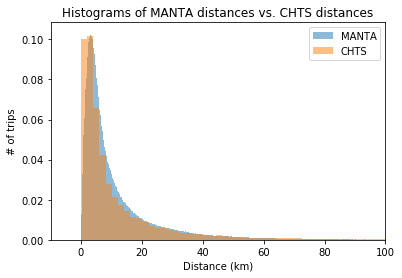
\includegraphics[width=.45\textwidth]{figs/manta_vs_chts_shortest_path.png}
    \caption{Comparison of trip lengths in MANTA versus California Household Travel Survey data. Median distance in MANTA is 6.46 km and in CHTS is 5.33 km.}
    \label{fig:distance}
\end{figure}

% \begin{figure}[H] 
%     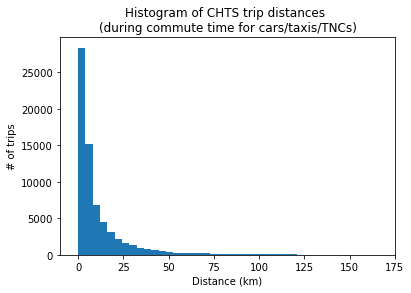
\includegraphics[width=.45\textwidth]{figs/chts_distances.png}
%     \caption{Distances traveled in CHTS data}
%     \label{fig:chts_distance}
% \end{figure}

The validation of the traffic microsimulator involves comparing the MANTA outputs to Uber Movement distributions at specific time slices. In particular, using Q2 Uber Movement data from 2019, 95,510 edges, or 17\%, of the total edges are matched to the Uber network.

One important enhancement is made to the simulator to better reflect vehicular behavior. In the IDM, $v_0$ represents the free-flow velocity of a vehicle on an edge, typically the speed limit of each edge from OSM or from a standard convention. However, in order to mimic the variance of driving patterns across travelers, each driver's maximum possible speed per edge, $v_0$, is sampled from a Gaussian distribution centered around the edge's predetermined speed limit with a standard deviation of $2\sigma_s$, where $\sigma_s$ is the standard deviation of vehicle speeds at each speed limit $s$. Every vehicle thus has a slightly different maximum allowable speed on each edge it traverses.

For the simulation run between 5 AM - 12 PM, the curves displayed are for 5 AM - 6 AM, a less congested time period, and 8 AM - 9 AM, a more congested time period. Within each time period, a subset of curves is presented at different speed limits. For instance,~\Cref{fig:kde_5to6_35} and ~\Cref{fig:kde_8to9_35} show the speed distributions from MANTA on edges with 35 mph compared to the Uber Movement data on those same edges, between 5 AM and 6 AM, and 8 AM and 9 AM, respectively. The figures confirm that both MANTA and Uber average speeds are higher between 5 AM and 6 AM than those between 8 AM and 9 AM.

\begin{figure}
    \centering
    \begin{subfigure}{\linewidth}
        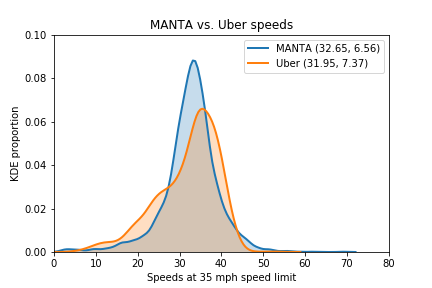
\includegraphics[width=\linewidth]{figs/green_lights_5to6/kde_plot_speed_35.png}
        \caption{5 AM - 6 AM}
        \label{fig:kde_5to6_35}
    \end{subfigure}\\
    \begin{subfigure}{\linewidth}
    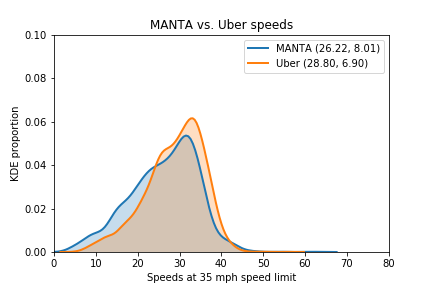
\includegraphics[width=\linewidth]{figs/green_lights_8to9/kde_plot_speed_35.png}
    \caption{8 AM - 9 AM}
    \label{fig:kde_8to9_35}
    \end{subfigure}
    \caption{Kernel density plot comparing the MANTA and Uber distributions at 35 mph}
\end{figure}

%The $r^2$ of .014 reflects a relatively close association between the two distributions in~\Cref{fig:reg_5to6_35}.

% \begin{figure}[H] 
%     \includegraphics[width=.45\textwidth]{green_lights_5to6/reg_plot_speed_35.png}
%     \caption{Regression plot comparing the MANTA and Uber distributions at 35 mph [5 AM - 6 AM], with an $r^2$ of .014 and the distributions in the previous plot shown on the axes}
%     \label{fig:reg_5to6_35}
% \end{figure}

\Cref{fig:avg_microsim_vs_uber_5to6} shows the average speeds of MANTA and Uber across all speed limits between 5 AM and 6 AM. At low-speed edges ($<$ 30 mph), MANTA simulation speeds are approximately 5 mph slower than Uber's real-world data. This indicates that the congestion effects are larger at lower speeds in MANTA. The Uber speeds also reflect that many drivers tend to go above the speed limits more so on edges with lower speed limits than they do on edges with higher speed limits. For edges with speed limits above 30 mph, MANTA and Uber estimates vary.

\begin{figure}
    \centering
    \begin{subfigure}{\linewidth}
        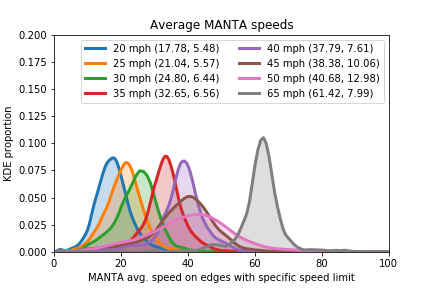
\includegraphics[width=\linewidth]{figs/green_lights_5to6/avg_MANTA_speeds.png}
    \end{subfigure}\\
    \begin{subfigure}{\linewidth}
        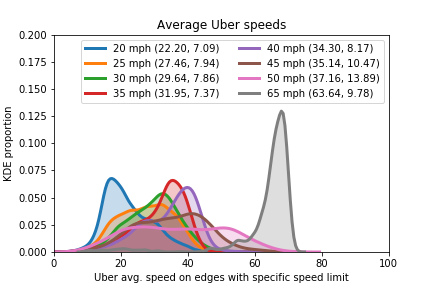
\includegraphics[width=\linewidth]{figs/green_lights_5to6/avg_uber_speeds.png}
    \end{subfigure}
    \caption{Average MANTA and Uber speeds across all speed limits [5 AM - 6 AM]. The means and standard deviations are shown in parentheses.}
    \label{fig:avg_microsim_vs_uber_5to6}
\end{figure}

The same plots are shown for the 8 AM - 9 AM timeframe in~\Cref{fig:avg_microsim_vs_uber_8to9}. Unlike in the 5 AM to 6 AM timeframe, MANTA simulation speeds are equal to or slower than Uber's real-world data across all speed limits. This indicates that MANTA may be overly sensitive to congestion effects.

\begin{figure}
    \centering
   \begin{subfigure}{\linewidth}
        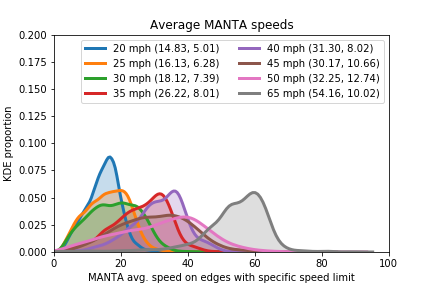
\includegraphics[width=\linewidth]{figs/green_lights_8to9/avg_MANTA_speeds.png}
    \end{subfigure}\\
    \begin{subfigure}{\linewidth}
        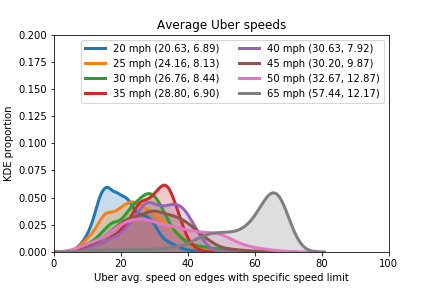
\includegraphics[width=\linewidth]{figs/green_lights_8to9/avg_uber_speeds.png}
    \end{subfigure}
    \caption{Average MANTA and Uber speeds across all speed limits [8 AM - 9 AM]. The means and standard deviations are shown in parentheses.}
    \label{fig:avg_microsim_vs_uber_8to9}
\end{figure}

Comparing the 5 AM - 6 AM timeslice with 8 AM - 9 AM in MANTA, the average speeds estimated in the early morning time period in general are higher by 3 to 9 mph across all speed limits, with the greater differences being on edges with higher speed limits. This intuitively suggests that higher speed roadways see less traffic at the early morning hours, and thus vehicles can travel at higher speeds due to the lack of congestion and lack of stoppage. However, roadways that have lower speed limits do not allow for much higher speeds regardless of the time of the day. This is likely due to the presence of frequent intersections in the city. The Uber data across the two timeslices also reflect this difference.

% \begin{figure}[H] 
%     \includegraphics[width=.45\textwidth]{figs/green_lights_8to9/reg_plot_speed_35.png}
%     \caption{Regression plot comparing the MANTA and Uber distributions at 35 mph [8AM-9AM], with an $r^2$ of .014 and the distributions in the previous plot shown on the axes}
%     \label{fig:reg_8to9_35}
% \end{figure}

% \begin{figure}[H] 
%     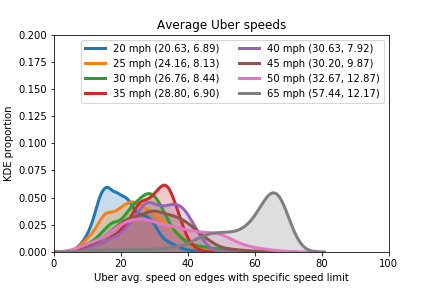
\includegraphics[width=.45\textwidth]{figs/green_lights_8to9/avg_uber_speeds.png}
%     \caption{Average Uber speeds across all speed limits [8AM-9AM]. The means and standard deviations are shown in parentheses.}
%     \label{fig:avg_uber_8to9}
% \end{figure}

\subsection{Red light / green light cases}
In this study, a basic intersection model is adopted with two conditions, where every node is either a red light or a green light. Between 5 AM - 6 AM, the average speed is 17.5 mph, while the speed decreases to 12.9 mph in the 8 AM - 9 AM timeslice, with each speed limit's distribution shown in ~\Cref{fig:velocities_red_light}. The reduction in speed between 8 AM and 9 AM suggests increased congestion, in comparison to the free-flowing traffic in the early morning between 5 AM - 6 AM. 

\begin{figure}
    \centering
    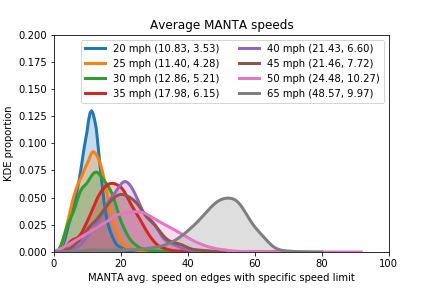
\includegraphics[width=0.49\textwidth]{figs/avg_vel_red_light_8to9.png}
    \caption{Average MANTA speeds across all speed limits [8 AM - 9 AM] in the red light case. The means and standard deviations are shown in parentheses.}
    \label{fig:velocities_red_light}
\end{figure}

When every node is a green light, the average speed across all speed limits from 5 AM - 6 AM is 24.5 mph, decreasing to 17.8 mph from 8 AM - 9 AM, whose distribution across speed limits is previously shown in~\Cref{fig:avg_microsim_vs_uber_8to9}. The difference in speed limit between the early morning timeslice and 8 AM - 9 AM time slice in the green light case is 4.6 mph, while in the red light condition, it is 6.7 mph. The deltas between the two timeslices, as well as the absolute speeds, highlight notable differences. Specifically, the average speeds in both timeslices under the red light condition is about 5 mph lower than the green light condition. Such low speeds are unsurprising given that every vehicle must stop and wait its turn in the intersection queue.


% In case 2, where every node is a green light, the average travel time decreases considerably to 36 minutes, median 11 minutes, and standard deviation 60 minutes, as shown in~\Cref{fig:travel_times_green_light}.

% \begin{figure}[H] 
% 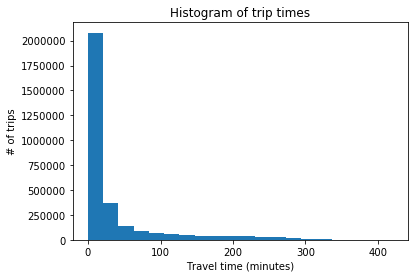
\includegraphics[width=.45\textwidth]{travel_times_green_light.png}
% \caption{Histogram of travel times in which each node is a green light}
% \label{fig:travel_times_green_light}
% \end{figure}

Notably, in~\Cref{fig:avg_microsim_vs_uber_8to9}, the lower speed limits' distributions tend to be right-skewed, following a lognormal pattern, while the distributions at higher speed limits become more centered and follow a normal distribution. Snapshots of these phenomena are shown in~\Cref{fig:lognormal_20_mph_green_light} and~\Cref{fig:normal_45_mph_green_light}.

\begin{figure}
    \centering
    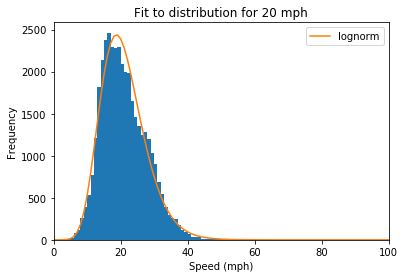
\includegraphics[width=.45\textwidth]{figs/lognormal_dist_20_mph_green_light.png}
    \caption{Fit to lognormal distribution for 20 mph speed limit in green light scenario (case 2)}
    \label{fig:lognormal_20_mph_green_light}
\end{figure}

\begin{figure}
    \centering
    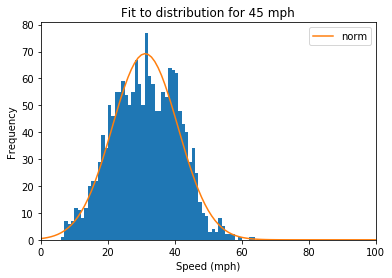
\includegraphics[width=.45\textwidth]{figs/normal_dist_45_mph_green_light.png}
    \caption{Fit to normal distribution for 45 mph speed limit in green light scenario (case 2)}
    \label{fig:normal_45_mph_green_light}
\end{figure}

The green light scenario was selected for calibration due to its closer alignment with the Uber data as well as its more accurate representation of highway travel.


\section{Performance benchmarks}

This section describes the profiling results of the two components of MANTA: shortest-path and simulation. 

\subsection{Shortest-path benchmarks}

In our network of approximately 225K nodes, 550K edges, and 3.2M OD pairs, the SSSP shortest-path algorithm carries out the computation of all OD pairs' routes in approximately 62 minutes on a single node.~\Cref{fig:time} shows the time-required to run up to 1 million agents on a distributed compute cluster utilizing both MPI and OpenMP parallelization schemes. The routing algorithm shows strong scaling that matches the theoretical scaling up to 1024 cores for routing 1 million agents. In comparison to existing routing algorithms, such as the heuristic-based Ligra~\cite{shun2013ligra} and iGraph~\cite{csardi2006igraph}, the priority-queue based Dijkstra is 2.2\% and 55\% faster, respectively, on a single node, as shown in~\Cref{fig:speedup}. The priority-queue Dijkstra algorithm also uses higher effective CPU usage of 94.1\% with an average RAM usage of 4.81 GB.

\begin{figure}
    \centering
    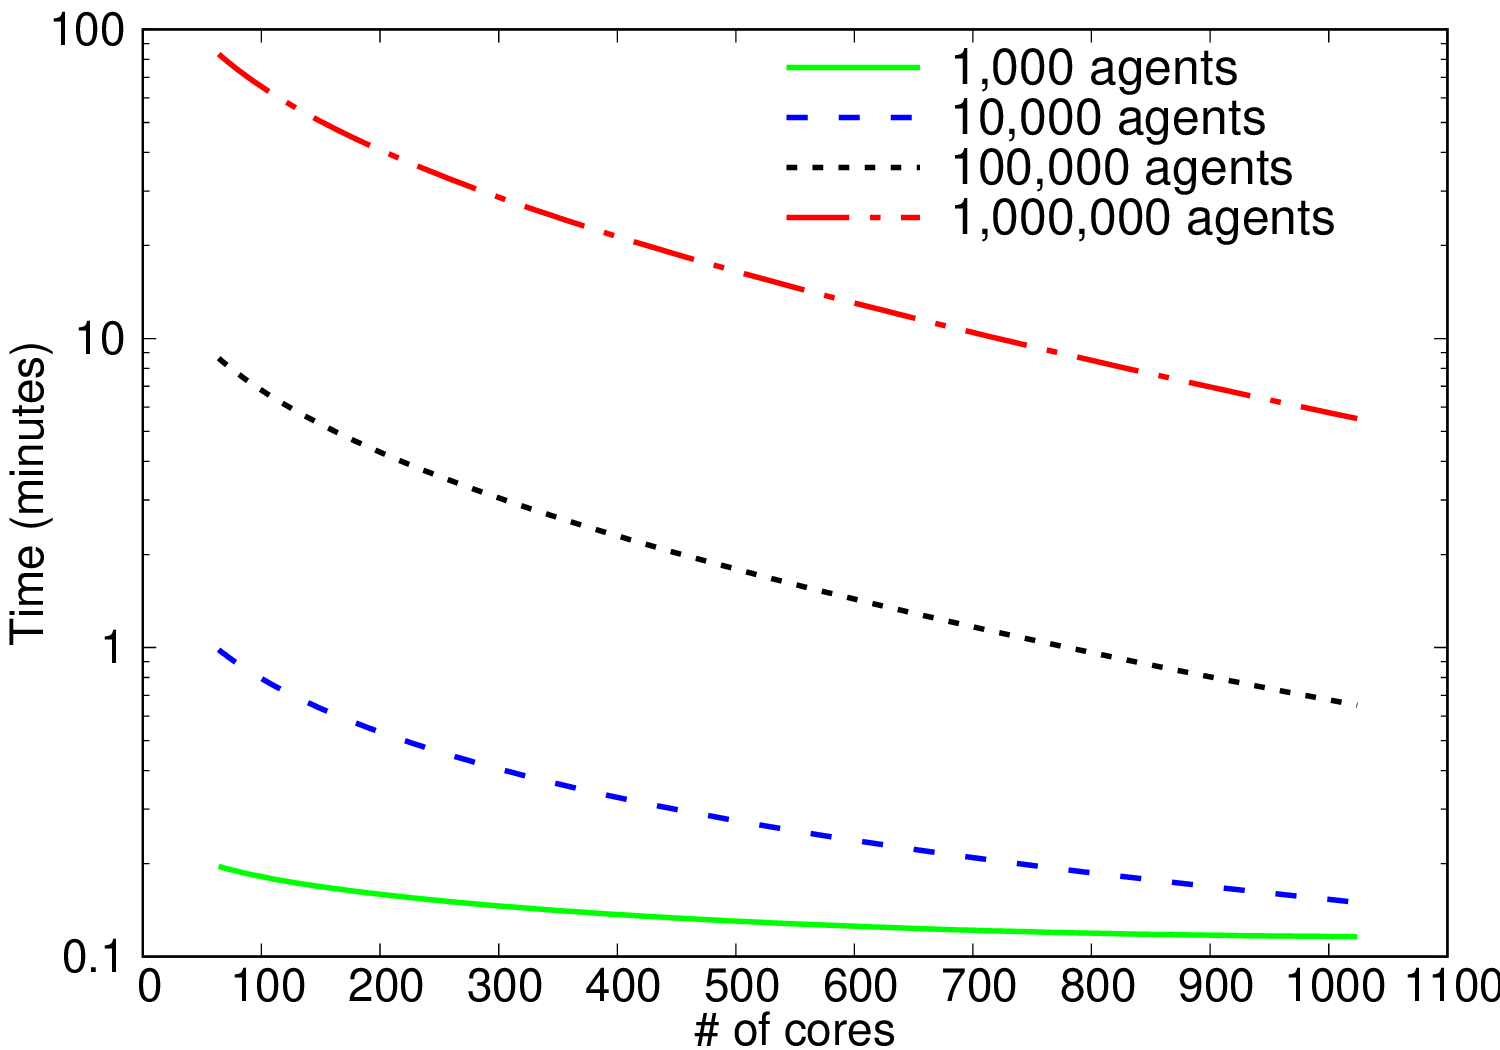
\includegraphics[width=\linewidth]{figs/time.png}
    \caption{Time required to route agents using priority-queue Dijkstra algorithm for the Bay-Area network on distributed computing environment (MPI + OpenMP) parallelization. Tests were run on 32 nodes with Intel Intel Xeon Skylake 6142 processors.}
    \label{fig:time}
\end{figure}

\begin{figure}
    \centering
    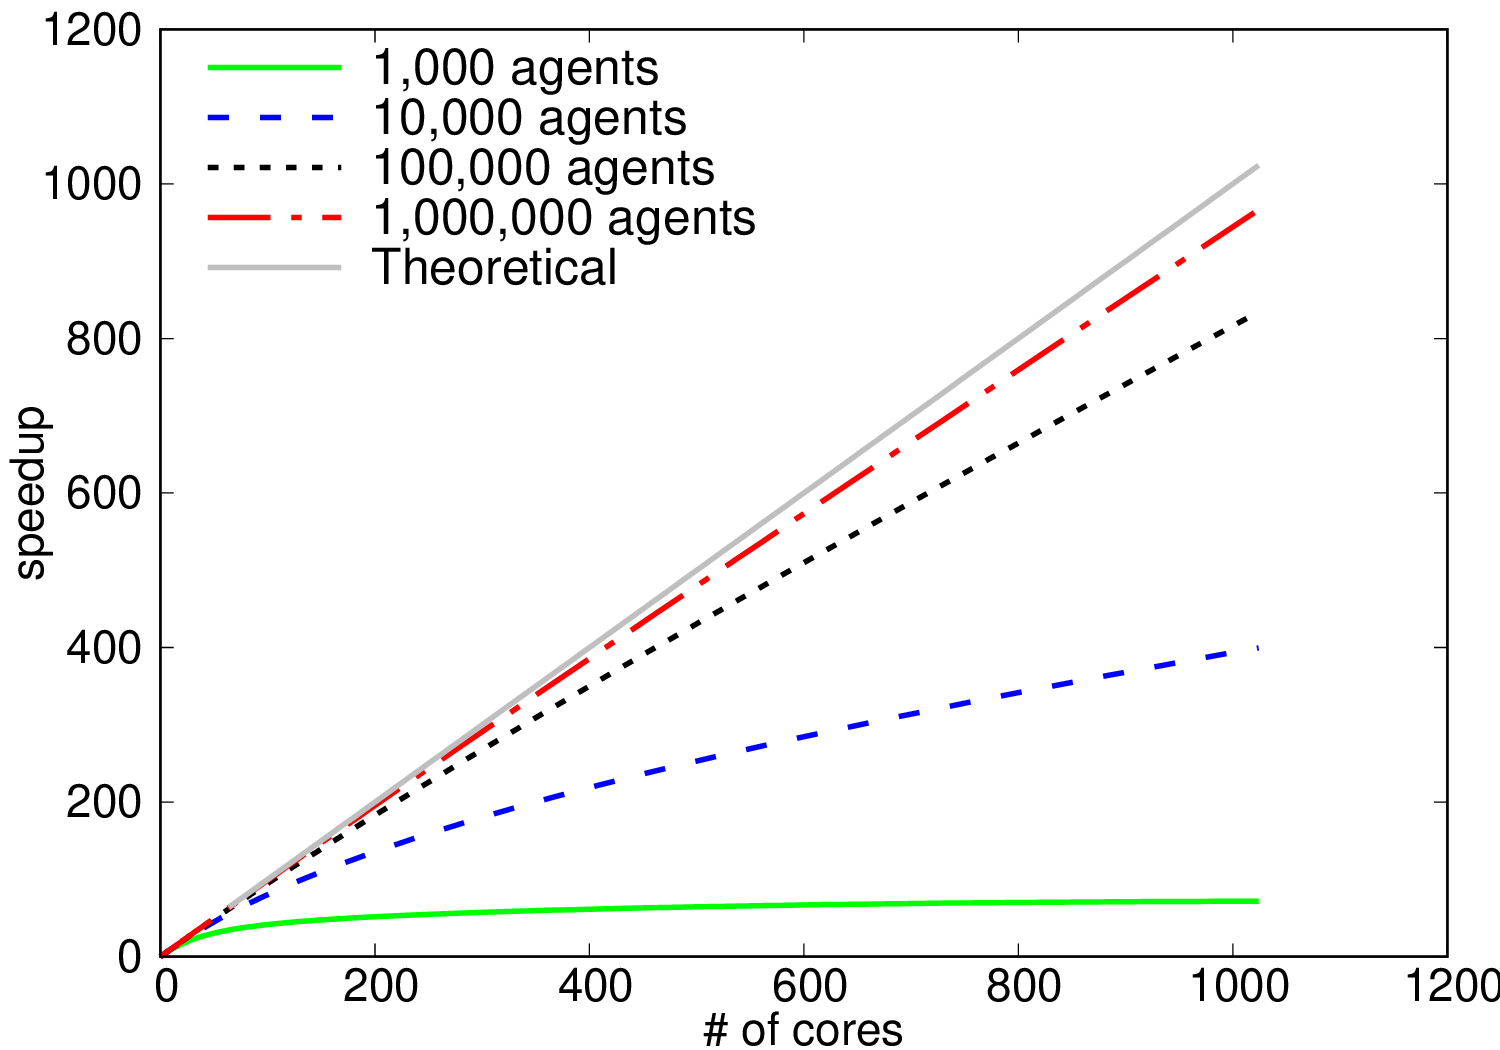
\includegraphics[width=\linewidth]{figs/speedup.png}
    \caption{Speedup of priority-queue routing algorithm for the Bay-Area network on distributed computing environment (MPI + OpenMP) parallelization. Tests were run on 32 nodes with Intel Intel Xeon Skylake 6142 processors.}
    \label{fig:speedup}
\end{figure}


%~\Cref{fig:shortest_path_runtimes} shows the general linearity of the SSSP priority queue algorithm as the demand increases from ~750K trips to 7.5M trips.

% \begin{figure}
%     \centering
%     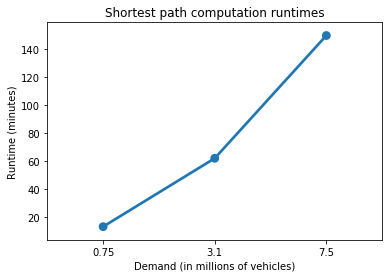
\includegraphics[width=.45\textwidth]{shortest_path_runtimes.png}
%     \caption{Shortest-path (routing) runtimes across different demands}
%     \label{fig:shortest_path_runtimes}
% \end{figure}

\subsection{Microsimulator benchmarks}

The computational performance of the MANTA simulator is compared with Simulation for Urban Mobility (SUMO) and JDEQSIM, a single-thread alternative available in MATSim, two well-known open-source simulators in transportation. The simulation of the Bay Area network and the demand between 5 AM - 12 PM are used for the comparison exercise. SUMO offers two options to build the network: one that contains internal links or lanes within intersections, and one that does not contain internal links~\cite{dlr46740}. Considering MANTA's simplified intersection model, the SUMO model without internal links is the most appropriate comparison. The SUMO model with internal links is also included for completeness but is only relevant for future iterations of MANTA that will include more advanced intersection control.

~\Cref{tab:runtimes} shows the runtime comparison of MANTA against SUMO and JDEQSIM. The table also indicates when the results are linearly extrapolated, due to the inability to complete simulations in a reasonable time. Extrapolating the simulation runtime linearly, MANTA performs nearly 27000x faster than SUMO. MANTA carried out the full microscopic simulation of 3.2M trips at .5 s timesteps in 4.6 minutes, while SUMO's simulator is estimated to take nearly 87 days, linearly extrapolated from the initial run of 194 minutes for 5000 trips. SUMO also has a mesoscopic simulator, which requires approximately 29 hours (1740 minutes) for the Bay Area simulation.

%However, mesoscopic does not give granular per-vehicle dynamics necessary for the highest integrity human and vehicle mobility patterns

A primary reason for such a dramatic difference in runtimes is that typically SUMO uses a traffic assignment model for routing. When the routes are fixed, as in this example, SUMO sees undesired jamming, as many roads are not filled to their capacities while other roads are filled excessively. The resulting congestion increases the simulation time in SUMO. While MANTA is not designed to produce an equilibrium assignment, it is able to manage fixed routes in a more manageable way than SUMO due to the scalable traffic atlas. Notably, SUMO's microsimulation does not support parallelization; only the routing algorithm is parallelized, which is not germane for this comparison.

JDEQSIM, developed at ETH Zurich, is an extension of MATSim integrated with BEAM, the modeling framework for Behavior, Energy, Autonomy, and Mobility, developed by Lawrence Berkeley National Laboratory. JDEQSIM achieves a level of granularity between cellular automata and mesoscopic simulation using event-based dynamics. However, it does not model granular movements at the microsimulation level, such as lane changing. \cite{waraichPerformanceImprovementsLargeScale2015}. 

~\Cref{fig:sim_runtime} shows the comparison of runtimes between JDEQSIM and MANTA. The JDEQSIM runtime is approximately 6.6 minutes, on average over 50 runs, and is comparable to MANTA's runtime of 4.6 minutes. The GPU parallelized traffic microsimulation in MANTA is 43\% faster than aggregated simulators such as JDEQSIM. In comparison to the SUMO microsimulation, MANTA is several orders of magnitude faster. Considering the finer level of behavioral granularity achieved by MANTA at the runtime of a mesoscopic simulator, these results clearly demonstrate the applicability of MANTA for regional-scale traffic microsimulations.

Other parallel microsimulators exist as well, including ~\cite{chanMobilitiScalableTransportation2018, barceloParallelizationMicroscopicTraffic1998, nagelParallelImplementationTRANSIMS2001}, but they either require expensive supercomputing machinery or carry out simulations on smaller networks with longer computation times.

\begin{table}
    \centering
    \begin{tabular}{l c c}
    \toprule
     \textbf{Simulator} & \textbf{Time (mins)} & \textbf{Type}\\
     \midrule
     MANTA & $4.6$ & Full\\
     SUMO meso simplified (MeS) & $1620$ & Full\\  %running right now
     SUMO micro simplified (MiS) & $114858$ & Lin. extrap.\\ %not done yet
     SUMO meso advanced (MeA) & $1740$ & Full\\
     SUMO micro advanced (MiA) & $123500$ & Lin. extrap.\\
     JDEQSIM & $6.6$ & Full\\
     \bottomrule
    \end{tabular}
    \label{tab:runtimes}
    \caption{MANTA's runtimes compared to SUMO and JDEQSIM. Full implies that the entire simulation was able to complete. Lin. extrap. implies that only part of the simulation was able to complete and the full time was linearly extrapolated from this preliminary time.}
\end{table}

\begin{figure}
    \centering
    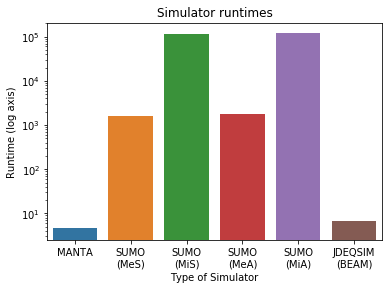
\includegraphics[width=.45\textwidth]{figs/sim_runtimes_log_y_axis.png}
    \caption{Simulator runtimes (log scale y-axis) across different simulators. MANTA performs slightly better than the parallelized mesoscopic JDEQSIM and is on the same order of magnitude. MANTA performs significantly better than the mesoscopic version of SUMO with either the simplified (MeS) or advanced intersection modeling (MeA). The microscopic version of SUMO with simplified intersections (MiS) and advanced intersections (MiA) could not be run completely, and thus times were linearly extrapolated, reflecting that it would take tens of days to complete.}
    \label{fig:sim_runtime}
\end{figure}



% We execute the subsequent microsimulation from 5 AM to 12 PM, producing benchmarks that vary across the timestep used, as shown in~\Cref{fig:microsim_benchmarks}. When looping over the range of timesteps from $[.1, .5, 1, 2, 10, 20]$ seconds, an inverse logarithmic pattern emerges, with .1 running for approximately 200 minutes (3.33 hours) .5 seconds taking 40 minutes, 1 second taking 20 minutes, 2 seconds taking 10 minutes, 10 seconds taking 2 minutes, and 20 seconds taking 1 minute.


% \begin{figure}[H] 
% 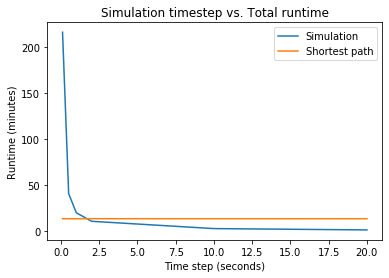
\includegraphics[width=.45\textwidth]{microsim_benchmarks.png}
% \caption{Microsimulator benchmarks across different timesteps}
% \label{fig:microsim_benchmarks}
% \end{figure}

% The simulation runtime (using a .5s timestep) must also be reviewed across different ranges of time. While 5 AM to 12 PM, or 7 hours, has been the standard simulation time, smaller simulation times have been considered, as low as 1 hour, as shown in~\Cref{fig:runtime_vs_timerange}

% \begin{figure}[H] 
% \includegraphics[width=.45\textwidth]{runtime_vs_time_range.png}
% \caption{Microsimulator runtime across different ranges of time}
% \label{fig:runtime_vs_timerange}
% \end{figure}

\section{Limitations and ongoing work}

The traffic microsimulation in MANTA achieves significant advances in computational performance using very large-scale networks and demand, but important limitations remain. The first limitation is the use of simplified intersection modeling. Although the simplification does not seem to have excessively impacted the validation results compared to real-world Uber Movement data, work is being conducted in traffic control inference using convolutional neural networks and vehicle trajectory data. We anticipate that accurate intersection modeling will produce more precise travel times and a better representation of the vehicle dynamics.

The second limitation is the demand profile. This work uses a synthetic Bay Area MTC 2017 travel model that represents the daily demand in five large time blocks and carries out a static traffic assignment. Future work involves tightly integrating MANTA with a dynamic travel demand model such as ActivitySim. The future versions of MANTA will also include dynamic routing. %In addition, broader integration efforts into activity-based land use simulation, which includes workplace and residential location choices as well as auto ownership and new mobility adoption, are underway.

%Drivers often change their routes and behavior based on time-varying congestion patterns~\cite{loderUnderstandingTrafficCapacity2019}. Ongoing work involves developing a modified version of dynamic routing. Specifically, in order to run the routing algorithm only once, we propose to generate 3 different routes for every OD pair using a subgraph of the original street graph. First, origin/destination nodes are selected in the subgraph closest to the origin/destination nodes in the original graph. Then, the routing is computed between the subgraph origin/destination nodes, $O_{s}$ to $D_{s}$, where $s$ is subgraph. Afterward, the routing is computed between the subgraph origin/destinations and the origin/destination nodes in the original graph, $O_{l}$ to $O_{s}$ and $D_{s}$ to $D_{l}$, where $l$ is local. Future work also involves using a warm start to improve computational efficiency \cite{levinWarmstartingDynamicTraffic2015}.

\section{Conclusions}

This paper presents a novel traffic microsimulator, MANTA, that addresses the challenges of accurate traffic microsimulation at the metropolitan-scale. MANTA is highly efficient and is capable of simulating real-world traffic demand with a fine level of granularity on large-scale networks. The runtime efficiency of MANTA is achieved by efficiently coupling a distributed CPU-parallelized shortest-path algorithm and a massively parallelized GPU simulation that utilizes a novel traffic atlas to map the spatial distribution of vehicles as contiguous bytes of memory. The capability of MANTA is demonstrated by simulating a typical morning workday of the nine-county Bay Area network with 550K edges and 225K nodes, and approximately 3.2M OD pairs. The shortest-path calculations are completed in 62 minutes, and a simulation of 7 hours from 5 AM to 12 PM with .5 second timesteps is completed in 4.6 minutes. This is several orders of magnitude faster than the state of the art microsimulators with similar hardware. Achieving compelling performance in both efficiency and accuracy, MANTA offers significant potential for fast scenario planning in both short- and long-term applications in metropolitan and regional-scale analysis. Ongoing enhancements include improved intersection control, incorporating dynamic traffic assignment, and tightly integrating activity demand. 

\section{Acknowledgements}

This report and the work described were sponsored by the U.S. Department of Energy (DOE) Vehicle Technologies Office (VTO) under the Systems and Modeling for Accelerated Research in Transportation (SMART) Mobility Laboratory Consortium, an initiative of the Energy Efficient Mobility Systems (EEMS) Program. The following DOE Office of Energy Efficiency and Renewable Energy (EERE) managers played important roles in establishing the project concept, advancing implementation, and providing ongoing guidance: David Anderson, Rachael Nealer, and Erin Boyd as well as Prasad Gupte. This work was funded by the U.S. Department of Energy Vehicle Technologies Office under Lawrence Berkeley National Laboratory Contract No. DE-AC02-05CH11231. The second author would like to than the generous support for Arup, UK for funding towards research on efficient routing algorithms.

The authors would like to give a special thanks to Kenichi Soga, Bingyu Zhao, and the cb-cities research group at the University of California, Berkeley and the University of Cambridge; Rashid Waraich, Artavazd Balayan, and the BEAM project team at Lawrence Berkeley National Laboratory; and the SUMO open-source team for remote simulation support.

\section{Appendix}
The source code for the microsimulator is available at \href{https://github.com/UDST/manta}{MANTA}, a module of the Urban Data Science Toolkit.


\bibliographystyle{ieeetr}
\bibliography{references.bib}
%\end{multicols}


\end{document}